\documentclass[UTF8]{article}
\usepackage{graphicx}
\usepackage{multirow}
\usepackage{booktabs}
\usepackage{latexsym}
\usepackage{indentfirst}
\setlength{\parindent}{2em}
\usepackage{color}
\definecolor{lbcolor}{rgb}{0.9,0.9,0.9}
\usepackage{listings}
\usepackage{ulem}
\lstset{backgroundcolor=\color{lbcolor}}
\lstset{keywordstyle=\color[rgb]{0,0,1}}
\lstset{commentstyle=\color[rgb]{0.133,0.545,0.133}}
\lstset{stringstyle=\color[rgb]{0.627,0.126,0.941}}
\lstset{language=Matlab}
\lstset{numbers=left}
\lstset{breaklines=true}
\usepackage{amsmath}
\author{\textbf{Lecturer: Wang Liwei}\\He Shuncheng\hspace{18pt}Yi Minzhen}
\title{Machine Learning: Scribe Note 4}
\begin{document}
\maketitle
\section{VC Theory}
\subsection{Review}
This lecture, we continued the topic of VC Theory. We perceive VC Dimension as a kind of \textbf{uniform convergence} over a set of indicator functions. Let us review the definition of VC Dimension.\\
\rule{\textwidth}{0.5pt}\par
\textbf{Definition}:\par
\vspace{9pt}
Say $d$ is the VC-dim of $\Phi$ ($\Phi$ is a set of indicator functions), if $\exists z_{1}, z_{2},\cdots,z_{d}$ such that\par
\begin{equation*}
|{(\phi(z_{1}),\cdots,\phi(z_{d}), \phi\in\Phi)}|=2^{d}
\end{equation*}\par
and there are \textbf{no} $z_{1},\cdots, z_{d}, z_{d+1}$ such that\par
\begin{equation*}
|{(\phi(z_{1}),\cdots,\phi(z_{d+1}), \phi\in\Phi)}|=2^{d+1}
\end{equation*}
\rule{\textwidth}{0.5pt}\par
\vspace{9pt}
Using Chernoff Ineq., we can get (no proof here)\par
\begin{equation*}
P(\sup_{\phi\in\Phi}|E\phi(z)-\frac{1}{n}\sum_{i=1}^{n}\phi(z)|\geq\varepsilon)\leq 4e^{-n\varepsilon^{2}/8}(\frac{en}{d})^{d}
\end{equation*}\par
Furthermore, we obtain a bound of $E\phi(z)$ by solving the inequality above. $\forall\delta>0$, with probability $1-\delta$ over the random draw of $z_{1}, z_{2},\cdots, z_{n}$,\par
\begin{equation*}
E\phi(z)\leq\frac{1}{n}\sum_{i=1}^{n}\phi(z_{i})+\mathcal{O}\left(\sqrt{\frac{d\log(\frac{n}{d})+\log(\frac{1}{\delta})}{n}}\right)
\end{equation*}\par
holds true simultaneously for all $\phi\in\Phi$.\par
\subsection{Empirical Risk Minimization (ERM)}
Given hypothesis space $\mathcal{H}$, find $f\in\mathcal{H}$ to minimize training error. This procedure is so-called ERM.\\
\rule{\textwidth}{0.5pt}\par
\textbf{Theorem}:\par
Let $\mathcal{H}$ be a hypothesis space $y=\{\pm 1\}$. Assume $VC(\mathcal{H})=d$. For any learning problem (i.e., any underlying distribution $D$ of the data), the classifier $\hat{f}$ returned by the ERM learning alg. satisfies with prob. $1-\delta$ over the random draw of a training set $S$ of size $n$,\par
\begin{equation*}
P_{D}(y\neq \hat{f}(x))\leq P_{S}(y\neq \hat{f}(x))+\mathcal{O}\left(\sqrt{\frac{d\log(\frac{n}{d})+\log(\frac{1}{\delta})}{n}}\right)
\end{equation*}
\rule{\textwidth}{0.5pt}\par
\vspace{9pt}
Note that $P_{D}(y\neq \hat{f}(x))$ refers to the generalization error and $P_{S}(y\neq \hat{f}(x))$ refers to the training error. If we denote\par
\begin{equation*}
f^{*}=\arg\!\min_{f\in\mathcal{H}}P_{D}(y\neq f(x))
\end{equation*}\par
we get\par
\begin{equation*}
P_{D}(y\neq \hat{f}(x))\leq P_{D}(y\neq f^{*}(x))+\mathcal{O}\left(\sqrt{\frac{d\log(\frac{n}{d})+\log(\frac{1}{\delta})}{n}}\right)
\end{equation*}\par
\section{Practical Learning Algorithms}
\subsection{Linear Classifier}
The problem of linear classification is described as follow:\\
\rule{\textwidth}{0.5pt}\par
\textbf{Input}: $x\in\mathcal{R}^{d}$\par
\textbf{Output}: $y=\{\pm1\}$\par
\textbf{Hypothesis Space}: $\mathcal{H}={(w,b)|w\in\mathcal{R}^{d}, b\in\mathcal{R}}$\par
\textbf{Classifier}: $f(x)=sgn(w^{T}x+b)$\\
\rule{\textwidth}{0.5pt}\par
\vspace{9pt}
It is trivial to infer that $VC(\mathcal{H})=d+1$ in this problem. The task to find a hyperplane is equivalent to this optimization problem:\par
\begin{eqnarray*}
 &\max_{w,b,t} &t \\
&s.t. &y_{i}(w^{T}x_{i}+b)\geq t,\forall i\in[n]\\
& &||w||=1
\end{eqnarray*}
A hyperplane that classifies all the training samples to the correct class exists when the solution of the optimization problem gives $t\geq 0$. In fact, it is a \textbf{large margin classifier} (see the figure below for the definition of margin).\par
\begin{figure*}[htbp]
\centerline{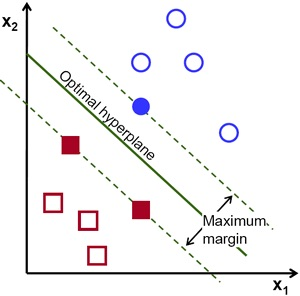
\includegraphics[width=2.5in]{optimal-hyperplane.jpg}}
\end{figure*}\par
Since we have algorithms to solve Linear Programming, Quadratic Programming, Convex Optimization and Semi-definite Programming, it is crucial to describe the problem in anothor way. The original programming is equivalent to a quadratic programming problem (its proof is left as exercise).\par
\begin{eqnarray*}
&\min_{w,b} & \frac{1}{2}||w||^{2}\\
&s.t. &y_{i}(w^{T}x_{i}+b)\geq 1,\forall i\in[n]
\end{eqnarray*}\par
Before we introduce the algorithm of this problem, the knowledge of Duality Theory is required.\par
\subsection{Minimax Theorem and Duality}
\subsubsection{Matrix Game}
\textbf{Pure strategy}\par
\vspace{9pt}
Consider a matrix $M=\{(m_{ij},\tilde{m}_{ij})\}_{s\times t}$ and two players, Row player and Column player. The Row player chooses one row first, the $i$th row for exapmle, and the Column player chooses one column (the $j$th column) seeing the Row player's move. Then, the Row player should pay $m_{ij}$ to Column and Column should pay $\tilde{m}_{ij}$ to Row. If matrix $M=\{m_{ij}\}_{s\times t}$, it is a zero-sum game, which means that Row should pay $m_{ij}$ to Column.\par
When Row takes the first move, they will reach\par
\begin{equation*}
\min_{i}\max_{j} m_{ij}
\end{equation*}\par
When Row takes the second move, they will reach\par
\begin{equation*}
\max_{j}\min_{i} m_{ij}
\end{equation*}\par
We have a conclusion that\par
\begin{equation*}
\min_{i}\max_{j} m_{ij}\geq\max_{j}\min_{i} m_{ij}
\end{equation*}\par
\textbf{Mixed strategy}\par
\vspace{9pt}
Row player chooses a distribution $p$ over $[s]$, and Column player, after seeing Row player's $p$, chooses a distribution $q$ over $[t]$.\par
When Row takes the first move, they will reach\par
\begin{equation*}
\min_{p}\max_{q}p^{T}Mq
\end{equation*}\par
When Row takes the second move, they will reach\par
\begin{equation*}
\max_{q}\min_{p}p^{T}Mq
\end{equation*}\par
And we have a theorem (Von Neuman Minimax Theorem)\par
\begin{equation*}
\min_{p}\max_{q}p^{T}Mq=\max_{q}\min_{p}p^{T}Mq
\end{equation*}
\rule{\textwidth}{0.5pt}\par
\textbf{Theorem 1}:\par
$\forall M=\{m_{ij}\}_{s\times t}$, $\exists p^{*},q^{*}$, such that $\forall p, q$\par
\begin{equation*}
p^{*T}Mq\leq p^{*T}Mq^{*}\leq p^{T}Mq^{*}
\end{equation*}\\
\rule{\textwidth}{0.5pt}\\
\vspace{9pt}
${}$\\
\rule{\textwidth}{0.5pt}\par
\textbf{Theorem 2}:\par
Function $f(x,y)$, $\forall y$, $f(\cdot,y)$ is convex, and $\forall x$, $f(x,\cdot)$ is concave\par
\begin{equation*}
\min_{x}\max_{y}f(x,y)=\max_{y}\min_{x}f(x,y)
\end{equation*}\par
and $(x^{*},y^{*})$ is saddle point.\\
\rule{\textwidth}{0.5pt}\par
\vspace{9pt}
\subsubsection{Lagrangian Duality}
A primal problem:\\
\rule{\textwidth}{0.5pt}\par
\textbf{Primal}:\par
\begin{eqnarray*}
 &\min_{x} &f(x) \\
&s.t. &g_{i}(x)\leq 0, \forall i\\
& &h_{j}(x)=0, \forall j
\end{eqnarray*}\par
$f$, $g_{i}$ are convex fuctions and $h_{j}$ are linear functions.\\
\rule{\textwidth}{0.5pt}\\
${}$\\
\rule{\textwidth}{0.5pt}\par
\textbf{Proposition 1}:\par
\begin{equation*}
\textbf{Primal}\Leftrightarrow
\min_{x}\max_{\lambda,\mu,\lambda\geq 0}f(x)+\sum_{i}\lambda_{i}g_{i}(x)+\sum_{j}\mu_{j}h_{j}(x)
\end{equation*}\par
Denote the target function with $L(x;\lambda,\mu)$\\
\rule{\textwidth}{0.5pt}\\
${}$\\
\rule{\textwidth}{0.5pt}\par
\textbf{Proposition 2}:\par
\begin{equation*}
\textbf{Primal}\Leftrightarrow
\max_{\lambda,\mu,\lambda\geq 0}f(\varphi)+\sum_{i}\lambda_{i}g_{i}(\varphi)+\sum_{j}\mu_{j}h_{j}(\varphi)
\end{equation*}\par
And\par
\begin{equation*}
\left.\frac{\partial L}{\partial x}\right|_{x=x^{*}}\Rightarrow x^{*}=\varphi(\lambda,\mu)
\end{equation*}\\
\rule{\textwidth}{0.5pt}\\
\section{Exercise}
\subsection{Ex 1}
Give a proof of\par
\begin{equation*}
VC(\mathcal{H})=VC(\Phi)
\end{equation*}
\subsection{Ex 2}
Prove the equivalence of the two optimization problems\par
\begin{eqnarray*}
 &\max_{w,b,t} &t \\
&s.t. &y_{i}(w^{T}x_{i}+b)\geq t,\forall i\in[n]\\
& &||w||=1
\end{eqnarray*}\par
and\par
\begin{eqnarray*}
&\min_{w,b} & \frac{1}{2}||w||^{2}\\
&s.t. &y_{i}(w^{T}x_{i}+b)\geq 1,\forall i\in[n]
\end{eqnarray*}
\subsection{Ex 3}
Give the dual problem of the latter one of \textbf{Ex 2}, namely the dual problem of\par
\begin{eqnarray*}
&\min_{w,b} & \frac{1}{2}||w||^{2}\\
&s.t. &y_{i}(w^{T}x_{i}+b)\geq 1,\forall i\in[n]
\end{eqnarray*}
\end{document}